

\فصل{راهنمای متن برنامک}

\begin{center}
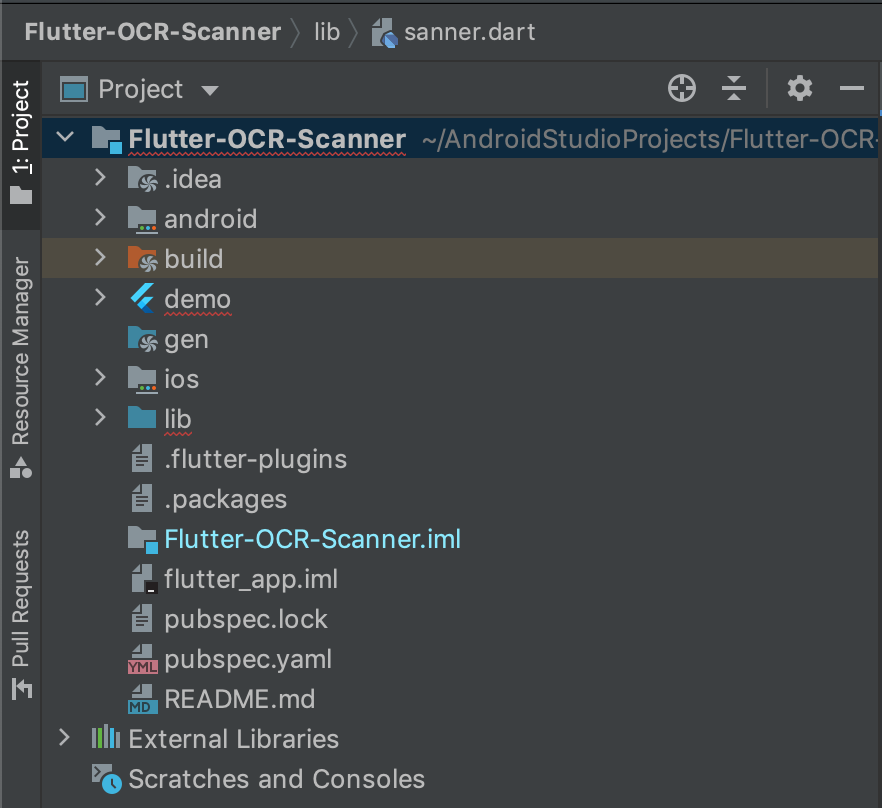
\includegraphics[scale=0.75]{front/template/images/packages.png}
\end{center}

منبع متن این برنامک بـر بسـتر ابـزار بازبینی نـسخه گیت‌‌هاب تـوسـعه داده شـده که مخـزن عـمومی آن را می‌توانید در آدرس پیوند \href{https://github.com/mahdihs76/drugdetector}{https://github.com/mahdihs76/drugdetector} مـشاهـده و بررسی کنید.

در این فصل بعضی از قسمت‌های مهم این متن را وارسی می‌کنیم.

\قسمت{کلاس TextDetectorPainter}
\شروع{شکل}[ht]
\begin{center}
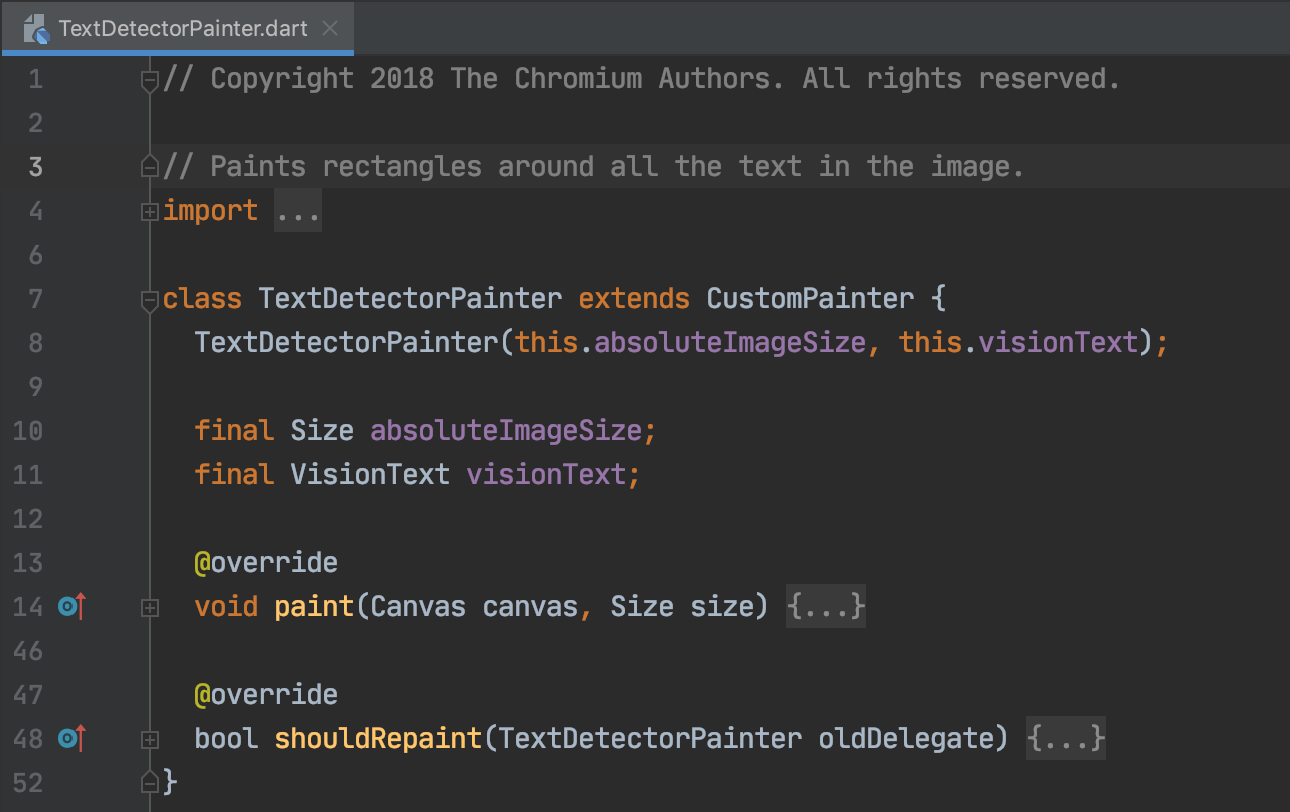
\includegraphics[scale=0.7]{front/template/images/text-painter.png}
\end{center}
\شرح{ساختار کلاس TextDetectorPainter}
\پایان{شکل}
در فـرآیند پویش جـعبه دارو، نیاز اسـت تـا بـا تشخیص مـحتواي متنی مـورد نـظر، آن را در لحـظه روي دوربین مـوبـایل مـشخص کنیم تـا کاربـر مـتوجـه شـود که قـسمت مـورد نـظر بـه درسـتی تشخیص داده شـده اسـت. 
\newline
TextDetectorPainer مـنطق این کار را بـرعهـده دارد و بـا اسـتفاده از سـه رنـگ سـبز، زرد و قـرمـز مـرز قـطعات مـشخص شـده روي دوربین را رسـم میکند.
\newline
 بـراي پیاده سـازي این کلاس از قـابلیت CustomPainter چـارچـوب فـلاتـر اسـتفاده میکنیم که قـابلیت هـرگـونـه ترسیم شخصی سازي شده را به توسعه دهنده می‌دهد.
 \newline
\شروع{شکل}[ht]
\begin{center}
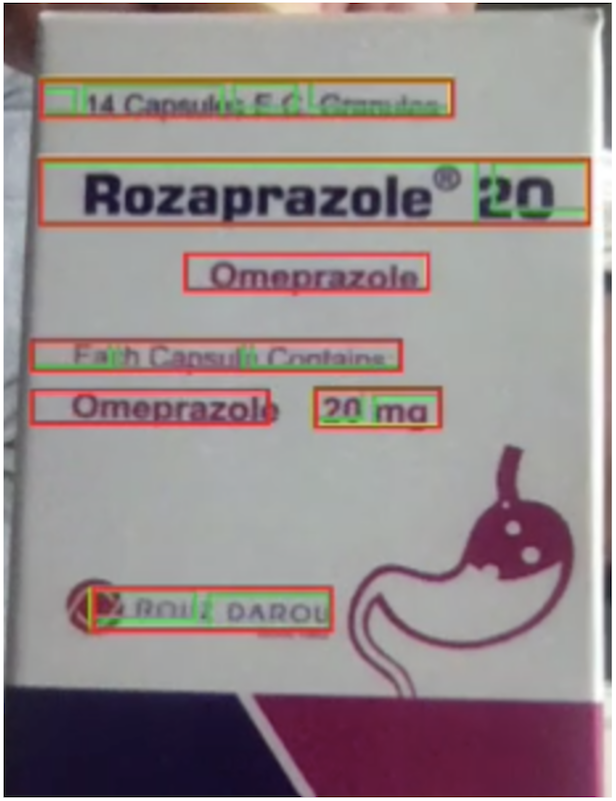
\includegraphics[scale=0.7]{front/template/images/text-detector.png}
\end{center}
\شرح{تشخیص مرز متون استخراج شده}
\پایان{شکل}


\قسمت{کلاس ScannerUtils}
\شروع{شکل}[ht]
\begin{center}
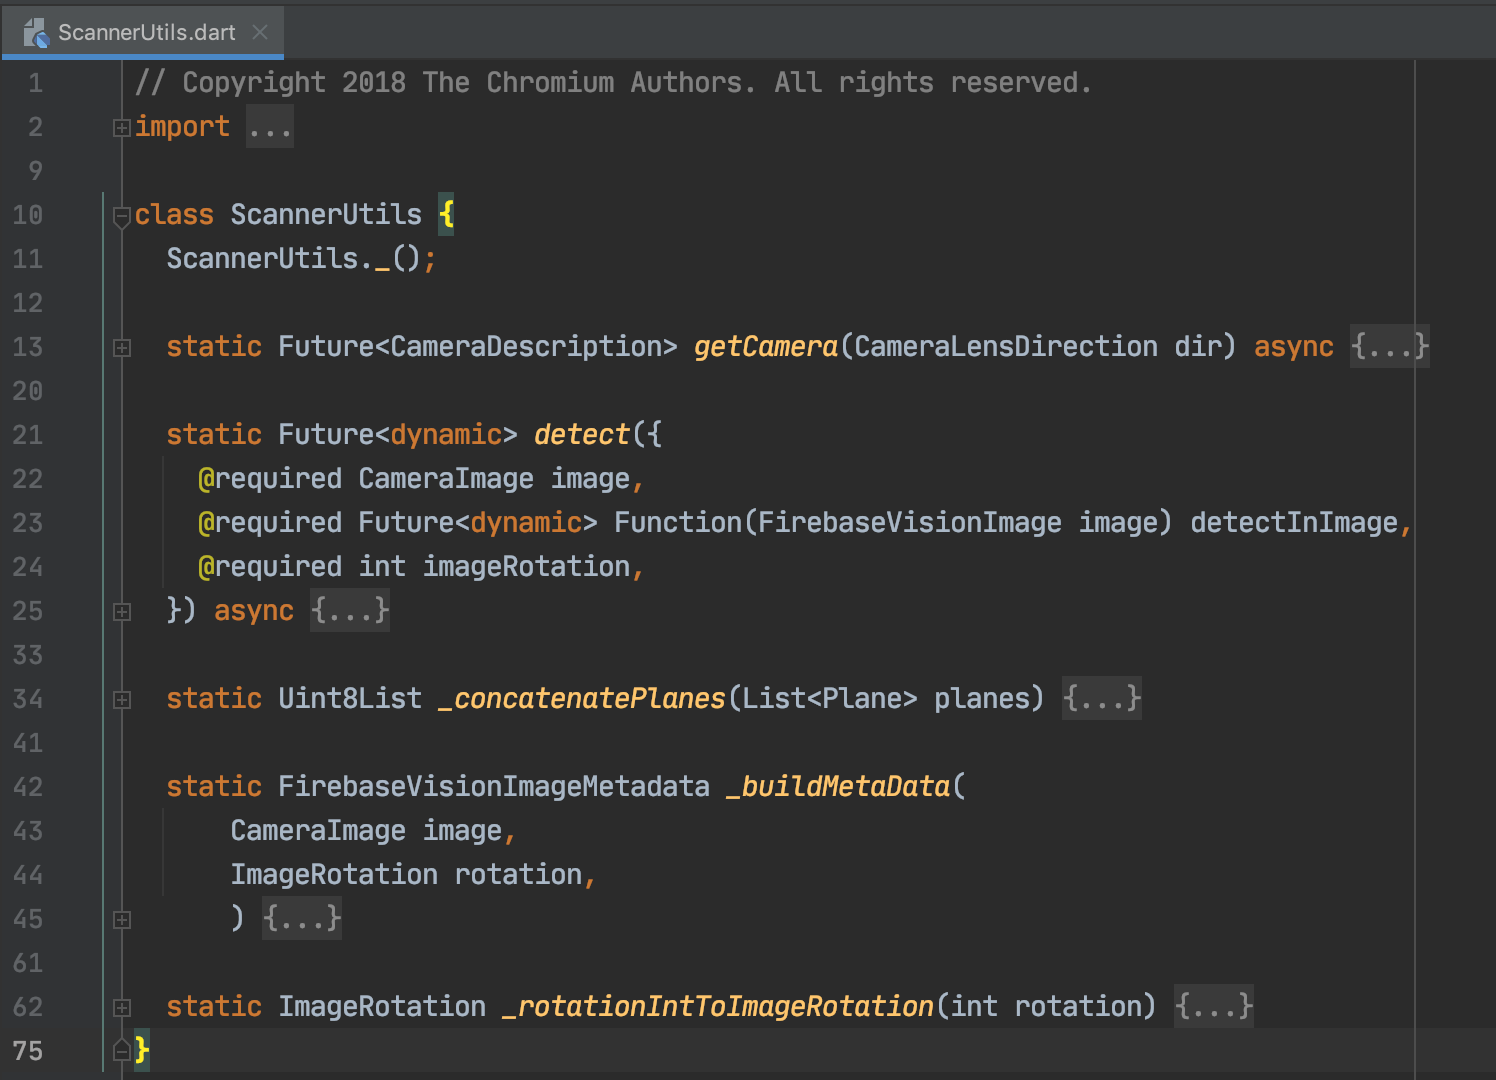
\includegraphics[scale=0.6]{front/template/images/scanner-utils.png}
\end{center}
\شرح{ساختار کلاس ScannerUtils}
\پایان{شکل}
این کلاس مـنطق عملکردي پـویشگر را مـدیریت میکند و تـوابعی را شـامـل میشـود که بـا در دسـت گرفتن دوربین موبایل به صورت لحظه اي متون پویش شده را بررسی کند.

\شروع{شمارش}
\فقره 
تابع getCamera : ابـتدا نیاز اسـت تـا بـا شـروع کار برنامک، دوربین مـوبـایل در دسـترس آن قـرار بگیرد. بـا فراخوانی این تابع، دوربین موبایل در اختیار برنامک ما قرار خواهد گرفت.
\فقره 
تابع detect : بـا فـراخـوانی این تـابـع، دوربین مـنتظر تشخیص مـتن روي جـعبه دارو خـواهـد مـانـد و بـلافـاصـله پـس ازتشخیص مـتن بـا اسـتفاده از یک Future در فـلاتـر (هـمانـند listener) برنامک را مـتوجـه این موضوع خواهد کرد.
\پایان{شمارش}

\قسمت{کلاس OCRPage}
\شروع{شکل}[ht]
\begin{center}
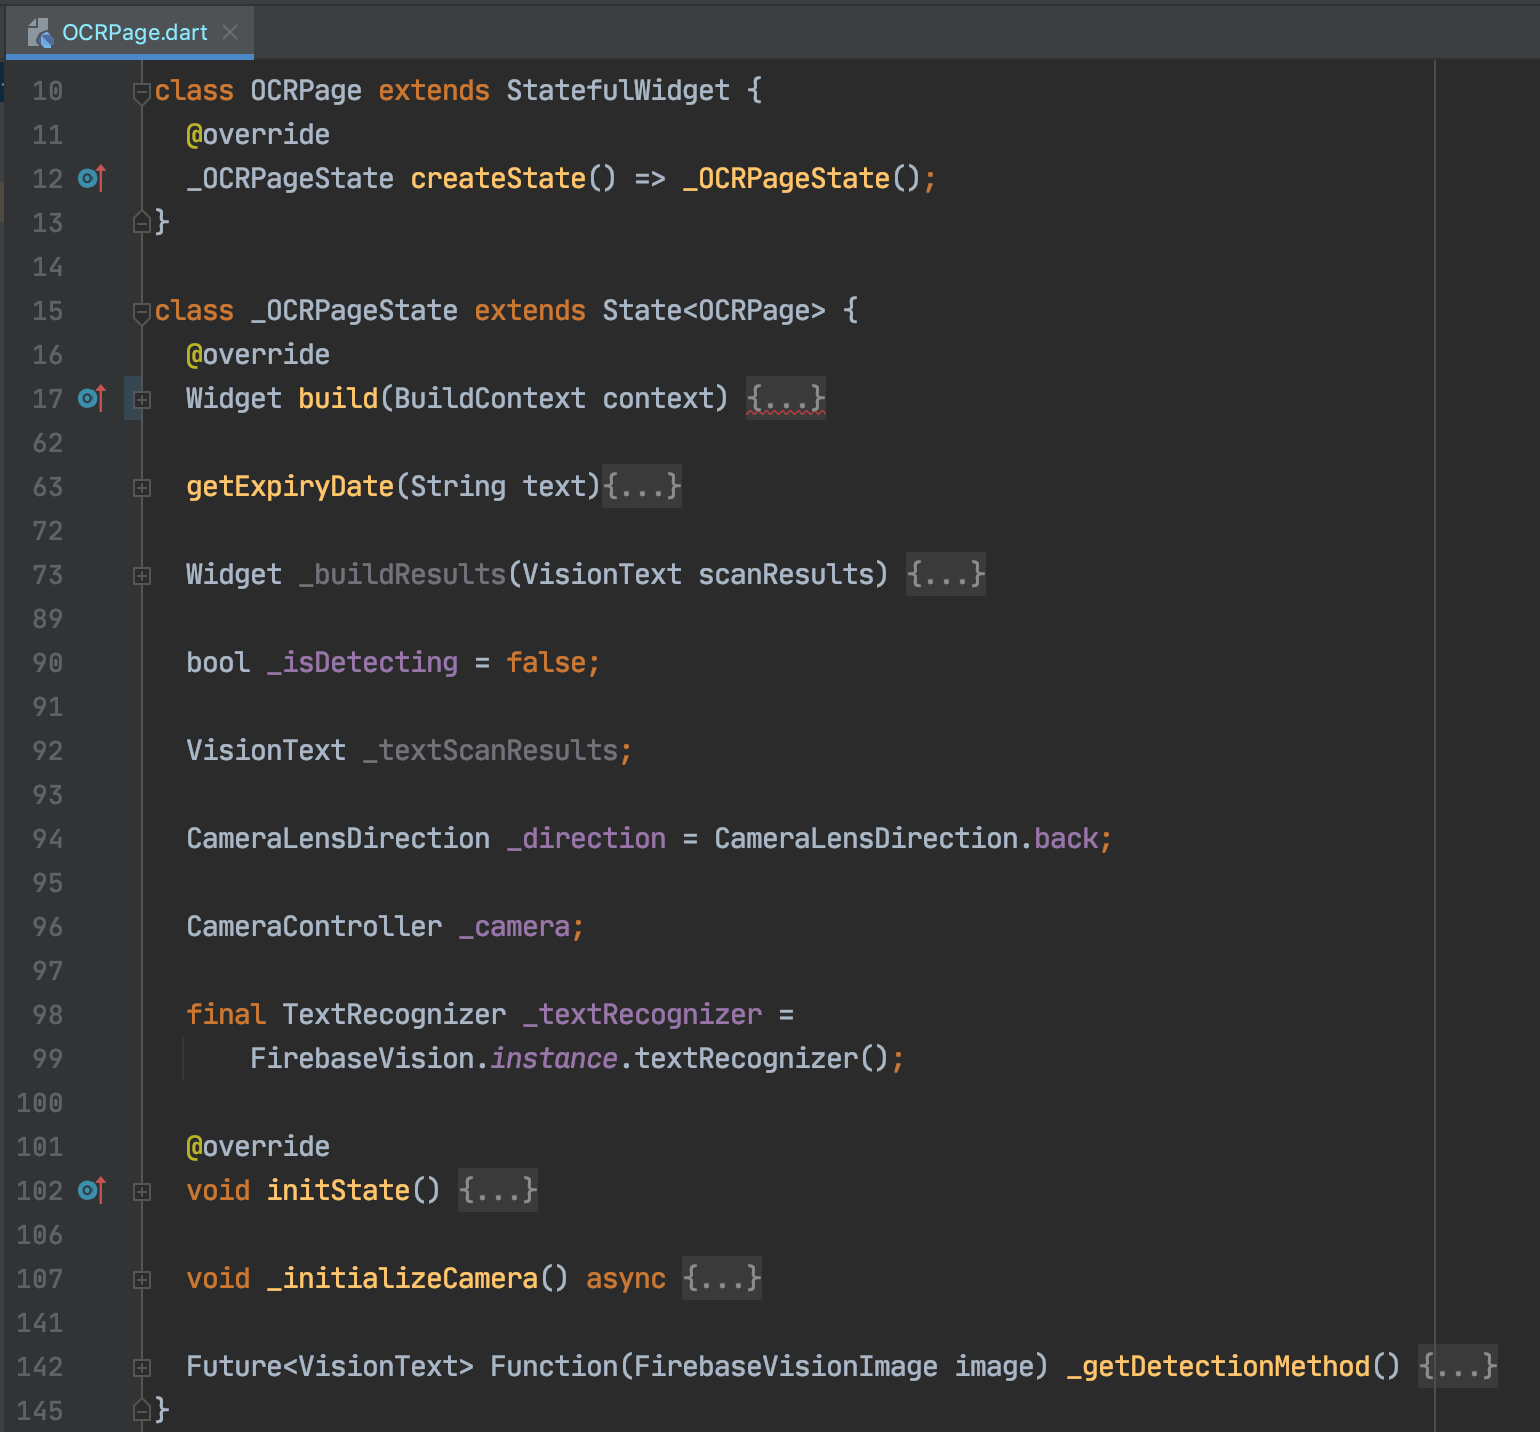
\includegraphics[scale=0.6]{front/template/images/ocr-page.png}
\end{center}
\شرح{ساختار کلاس OCRPage}
\پایان{شکل}
این کلاس صــفحه اصلی برنامک اســت که وظیفه اتــصال بــه دوربین مــوبــایل و مــنطق اصلی استخراج اطلاعات مورد نیاز دارو را برعهده دارد.
بـراي مـثال یکی از تـوابـع این کلاس، تـابـع getExpiryDate اسـت که بـا اسـتفاده از Regex تاریخ انقضاي دارو را استخراج میکند.

\شروع{شکل}[ht]
\begin{center}
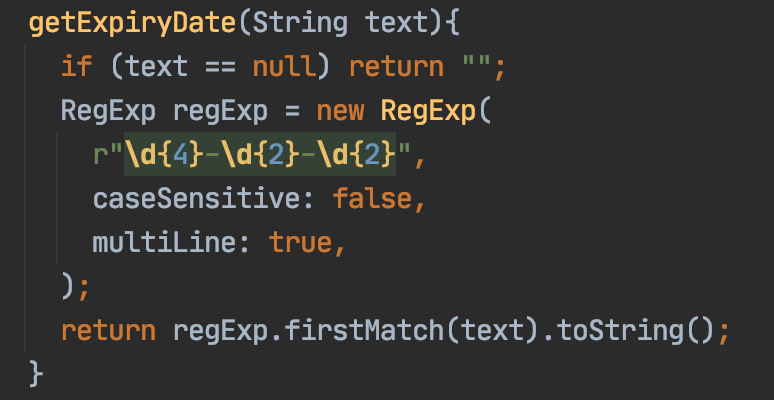
\includegraphics[scale=0.6]{front/template/images/get-expiry-date.png}
\end{center}
\شرح{منطق تشخیص تاریخ انقضا با استفاده از Regex }
\پایان{شکل}
